%-------------------------
% Matteo Dante - Public Summary CV (EN)
% Template: Harshibar (MIT) - adapted
%-------------------------

\documentclass[a4paper,10pt]{article}

\usepackage{latexsym}
\usepackage[a4paper,margin=12mm]{geometry}
\usepackage{titlesec}
\usepackage{marvosym}
\usepackage[usenames,dvipsnames]{color}
\usepackage{verbatim}
\usepackage{enumitem}
\usepackage[hidelinks]{hyperref}
\usepackage{fancyhdr}
\usepackage[english]{babel}
\usepackage{tabularx}
\usepackage{graphicx}


\definecolor{light-grey}{gray}{0.83}
\definecolor{dark-grey}{gray}{0.3}
\definecolor{text-grey}{gray}{.08}

\DeclareRobustCommand{\ebseries}{\fontseries{eb}\selectfont}
\DeclareTextFontCommand{\texteb}{\ebseries}

\usepackage[normalem]{ulem}
\renewcommand{\ULdepth}{1.8pt}
\newcommand{\myuline}[1]{\uline{#1}}

\usepackage{tgheros}
\renewcommand*\familydefault{\sfdefault}
\usepackage[T1]{fontenc}
\renewcommand{\small}{\fontsize{9.5}{11.5}\selectfont}
\hypersetup{pdftitle={Matteo Dante - CV},pdfauthor={Matteo Dante}}

\graphicspath{{../images/}}

\pagestyle{fancy}
\fancyhf{}
\fancyfoot{}
\renewcommand{\headrulewidth}{0pt}
\renewcommand{\footrulewidth}{0pt}

\setlength{\footskip}{4pt}

\urlstyle{same}

\raggedbottom
\raggedright
\setlength{\tabcolsep}{0in}

\titleformat{\section}{
    \bfseries \raggedright \large
}{}{0em}{}[\color{light-grey}{\titlerule[2pt]} \vspace{-4pt}]
\titlespacing*{\section}{0pt}{6pt}{5pt}

\newcommand{\resumeItem}[1]{
  \item\small{
    {#1 \vspace{-1pt}}
  }
}

\newcommand{\resumeSubheading}[4]{
  \vspace{-1pt}\item
    \begin{tabular*}{\textwidth}[t]{l@{\extracolsep{\fill}}r}
      \textbf{#1} & {\color{dark-grey}\small #2}\vspace{1pt}\\
      \textit{#3} & {\color{dark-grey} \small #4}\\
    \end{tabular*}\vspace{-4pt}
}

\renewcommand\labelitemii{$\vcenter{\hbox{\tiny$\bullet$}}$}

\newcommand{\resumeSubHeadingListStart}{\begin{itemize}[leftmargin=0in, label={},itemsep=3pt,topsep=2pt]}
\newcommand{\resumeSubHeadingListEnd}{\end{itemize}}
\newcommand{\resumeItemListStart}{\begin{itemize}[itemsep=1pt,topsep=3pt]}
\newcommand{\resumeItemListEnd}{\end{itemize}\vspace{0pt}}

\color{text-grey}

\begin{document}

%----------HEADER----------
\begin{minipage}[c]{0.13\textwidth}
  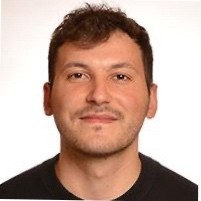
\includegraphics[width=\linewidth]{profile-pic.jpeg}
\end{minipage}\hfill
\begin{minipage}[c]{0.85\textwidth}
  \raggedright
  {\Huge \textbf{Matteo Dante}}\\[4pt]
  {\large Senior Software Engineer \textperiodcentered{} Full-Stack \& Backend}\\[6pt]
  \small
  \Email\ \href{mailto:matteo.dante659@gmail.com}{\texttt{matteo.dante659@gmail.com}} \hspace{4pt}$|$\hspace{4pt}
  \Mundus\ \href{https://matteodante.it}{\myuline{matteodante.it}}\\
  GitHub: \href{https://github.com/matteodante}{\myuline{matteodante}} \hspace{4pt}$|$\hspace{4pt}
  LinkedIn: \href{https://linkedin.com/in/matteo-dante-3705b5164}{\myuline{matteo-dante}} \hspace{4pt}$|$\hspace{4pt}
  Switzerland
\end{minipage}

\vspace{4pt}

\section{SUMMARY}
\small
Senior software engineer with 8+ years across aviation, high-traffic consumer platforms and retail. Builds web applications, backend services and AI products. Personal work includes two App Store apps and open-source tools for document retrieval, agents and self-hosted services.
\par\vspace{3pt}\textit{Public summary. Request access to the detailed CV via email or LinkedIn.}
\section{EXPERIENCE}
\resumeSubHeadingListStart
\resumeSubheading{Pilatus Aircraft Ltd}{04/2024 -- Present}{Senior Full-Stack Software Engineer}{Switzerland}
\resumeSubheading{DonTouch SA}{07/2023 -- 04/2024}{Backend Engineer}{Switzerland}
\resumeSubheading{Hexa Credit Care}{11/2019 -- 07/2023}{Full-Stack Developer}{Italy}
\resumeSubheading{Galileo SpA}{03/2018 -- 11/2019}{Full-Stack Developer}{Italy}
\resumeSubHeadingListEnd
\section{PERSONAL PROJECTS}
\small
\textbf{\href{https://apps.apple.com/us/app/maestro-learn-anything/id6780267046?uo=4}{Maestro}} -- Native iOS AI tutor on the App Store: source-grounded lessons, quizzes and tutor chat. SwiftUI, SwiftData, Hono, PostgreSQL.\\[3pt]
\textbf{\href{https://apps.apple.com/us/app/gymtree-workout-ai-coach/id6761392403?uo=4}{GymTree}} -- Fitness app on the App Store: backend, coach web, mobile app, subscriptions and AI coach. TypeScript, Expo, PostgreSQL, Redis, BullMQ.\\[3pt]
\textbf{\href{https://github.com/matteodante/claude-local-docs}{claude-local-docs}} -- MCP server for local documentation and code retrieval: hybrid search, reranking, AST-aware chunking and incremental indexing. TypeScript, LanceDB.\\[3pt]
\textbf{\href{https://github.com/matteodante/miniform}{Miniform}} -- Self-hosted form inbox with uploads, webhook/email retries and SQLite storage. Go, Docker; unit, integration and Playwright tests.\\[3pt]
\textbf{\href{https://github.com/matteodante/therapist}{Therapist}} -- Experimental self-reflection agent with encrypted memory, tool calling, validated outputs and regression tests. Python, PydanticAI.\\[3pt]
\textbf{\href{https://matteodante.it}{matteodante.it}} -- Interactive portfolio and playable CV with a streaming AI assistant. Next.js, vanilla Three.js, OpenAI Responses API; English/Italian.
\section{SKILLS}
\small
\textbf{Web \& backend}: TypeScript, Node.js, PHP, .NET, Java; React, Next.js, Laravel, Hono, REST, microfrontends\\[2pt]
\textbf{Personal projects}: Go, Python, Swift/SwiftUI, React Native (Expo), Three.js/WebGL\\[2pt]
\textbf{Data \& infrastructure}: PostgreSQL, MySQL, SQL Server, SQLite, Redis, BullMQ; Docker, Vercel, Railway, on-premise\\[2pt]
\textbf{AI \& retrieval}: OpenAI/Anthropic APIs, tool calling, MCP, structured outputs, streaming, RAG, BM25, RRF, reranking\\[2pt]
\textbf{Quality \& security}: Vitest, Bun test, pytest, Go tests, Playwright, CI; Sentry, OAuth/JWT\\[2pt]
\textbf{AI-assisted development}: Claude Code, Codex, Cursor; code review and automated checks
\section{EDUCATION \& LANGUAGES}
\small
Computer Science, Unitelma Sapienza, Rome, 2018--2021 (degree not completed).\\[2pt]
Diploma in Business Information Systems, Istituto E. Fermi, 2017. Italian: native; English: professional, daily use.
\end{document}
